%!TEX TS-program = xelatex
%!TEX encoding = UTF-8 Unicode
%!BIB TS-program = bibtex
%!TeX spellcheck = en_US
\documentclass[12pt]{article}
\usepackage[english]{babel}
\usepackage{url}
\usepackage[utf8x]{inputenc}
\usepackage{amsmath}
\usepackage{graphicx}
\graphicspath{{images/}}
\usepackage{parskip}
\usepackage{fancyhdr}
\usepackage{vmargin}
\usepackage{enumerate}
\usepackage[T1]{fontenc}
\usepackage{newpxtext,newpxmath}
\usepackage{booktabs}
\usepackage{siunitx}
\usepackage[version=4]{mhchem}
\usepackage{hyperref}
\usepackage{bm}
\usepackage{breqn}
\usepackage{miller}


\setmarginsrb{1 cm}{2.5 cm}{1 cm}{2.5 cm}{1 cm}{1.5 cm}{1 cm}{1.5 cm}
\sisetup{inter-unit-product = \ensuremath{{}\cdot{}}}
\DeclareTextCommand{\nobreakspace}{T1}{\leavevmode\nobreak\ }

\title{Solid State Physics HW 5}								% Title
\author{XYZ}								% Author
\date{}											% Date

\makeatletter
\let\thetitle\@title
\let\theauthor\@author
\let\thedate\@date
\makeatother

\pagestyle{fancy}
\fancyhf{}
\rhead{\theauthor}
\lhead{\thetitle}
\cfoot{\thepage}

\newcommand*{\rmn}[1]{\romannumeral#1}
\newcommand*{\RMN}[1]{\uppercase\expandafter{\romannumeral#1}}
 \newenvironment{mpmatrix}{\begin{medsize}\begin{pmatrix}}%
                {\end{pmatrix}\end{medsize}}%
\begin{document}

%%%%%%%%%%%%%%%%%%%%%%%%%%%%%%%%%%%%%%%%%%%%%%%%%%%%%%%%%%%%%%%%%%%%%%%%%%%%%%%%%%%%%%%%%

\begin{titlepage}
	\centering
	\vspace*{0.5 cm}
	
\includegraphics[scale = 0.25]{NewEngineeringDkBlue.png}\\[1.0 cm]	% University Logo
	\textsc{\Large Applied Physics and Applied Mathematics\\
		\large with Materials Science and Engineering}\\[2.0 cm]	% University Name
	\textsc{\Large APPH 6081}\\[0.5 cm]				% Course Code
	\rule{\linewidth}{0.2 mm} \\[0.4 cm]
	{ \huge \bfseries \thetitle}\\
	\rule{\linewidth}{0.2 mm} \\[1.5 cm]

	\begin{minipage}{0.4\textwidth}
		\begin{flushleft} \large
			\emph{Submitted To:}\\
			Chris Marianetti\\
			Assoc. Professor\\
			APAM Department\\
		\end{flushleft}
	\end{minipage}~
	\begin{minipage}{0.4\textwidth}

		\begin{flushright} \large
			\emph{Submitted By :} \\
			XYZ\\
			\texttt{xyz}\\
			Fall 2016\\
		\end{flushright}

	\end{minipage}\\[2 cm]


\end{titlepage}

\section*{Problem \RMN{1}}
\begin{enumerate}[(a)]
	\item
	      Suppose
	      \begin{equation}
	      	V(\bm{r}) = \sum_{\bm{G}} V_{\bm{G}} e^{i\bm{G}\cdot \bm{r}},
	      \end{equation}
	      where $V_{\bm{G}} = \int V(\bm{r})e^{-i\bm{G}\cdot\bm{r}} \, d\bm{r}$. Since we have liberty to add a constant to $V(\bm{r})$, we can always make $V_{\bm{G}=\bm{0}} = V_{(0,0)}=0$. We will use this proposition as default.
	      Here $V(\bm{r})$ can be expressed as
	      \begin{equation}
	      	V(\bm{r}) = \sum_{m_1, m_2} V_{(m_1, m_2)} e^{i (m_1 \bm{b}_1 + m_2 \bm{b}_2) \cdot \bm{r}},
	      \end{equation}
	      For direction $\hkl[1 0]$, $\bm{r}_1 = x\bm{a}_1 + 0\bm{a}_2$.
	      So
	      \begin{equation}
	      	\begin{split}
	      		V(\bm{r}_1) &= V_{(0,0)} e^{i 2\pi (0,0)\cdot (x,0)}  + V_{(1,0)} e^{i 2\pi (1,0)\cdot (x,0)} \\
	      		&+ V_{(1,0)} e^{i 2\pi (-1, 0)\cdot (x,0)} + V_{(0, 1)} e^{i 2\pi (0, 1)\cdot (x,0)} \\
	      		&+ V_{(0, -1)} e^{i 2\pi (0, -1)\cdot (x,0)} + V_{(1,1)} e^{i 2\pi (1, 1)\cdot (x,0)}\\
	      		&+ V_{(-1,-1)} e^{i 2\pi (-1, -1)\cdot (x,0)} + V_{(1,-1)} e^{i 2\pi (1,-1)\cdot (x,0)} \\
	      		&+ V_{(-1,1)} e^{i 2\pi (-1,1)\cdot (x,0)} \\
	      		&= \frac{\hbar^2}{2m}\frac{4\pi^2}{a^2}(0 -0.04 e^{-2 i \pi  x}-0.04 e^{2 i \pi  x}-0.08 -0.04 e^{-2 i \pi  x}-0.04 e^{2 i \pi  x})\\
	      		&= \frac{\hbar^2}{2m}\frac{4\pi^2}{a^2}(-0.16 \cos (2 \pi  x)-0.08).
	      	\end{split}
	      \end{equation}
	      For direction $\hkl[1 1]$, $\bm{r}_2 = x\bm{a}_1 + x\bm{a}_2$. So
	      \begin{equation}
	      	\begin{split}
	      		V(\bm{r}_2) &=  V_{(0,0)} e^{i 2\pi (0,0)\cdot (x,x)}  + V_{(1,0)} e^{i 2\pi (1,0)\cdot (x,x)} \\
	      		&+ V_{(1,0)} e^{i 2\pi (-1, 0)\cdot (x,x)} + V_{(0, 1)} e^{i 2\pi (0, 1)\cdot (x,x)} \\
	      		&+ V_{(0, -1)} e^{i 2\pi (0, -1)\cdot (x,x)} + V_{(1,1)} e^{i 2\pi (1, 1)\cdot (x,x)}\\
	      		&+ V_{(-1,-1)} e^{i 2\pi (-1, -1)\cdot (x,x)} + V_{(1,-1)} e^{i 2\pi (1,-1)\cdot (x,x)} \\
	      		&+ V_{(-1,1)} e^{i 2\pi (-1,1)\cdot (x,x)} \\
	      		&= \frac{\hbar^2}{2m}\frac{4\pi^2}{a^2}(0 -0.08 e^{-2 i \pi  x}-0.08 e^{2 i \pi  x} -0.02 e^{-4 i \pi  x}-0.02 e^{4 i \pi  x}-0.04) \\
	      		&= \frac{\hbar^2}{2m}\frac{4\pi^2}{a^2}(-0.16 \cos (2 \pi  x)-0.04 \cos (4 \pi  x)-0.04).
	      	\end{split}
	      \end{equation}
	      \begin{figure}[h]
	      	\centering
	      	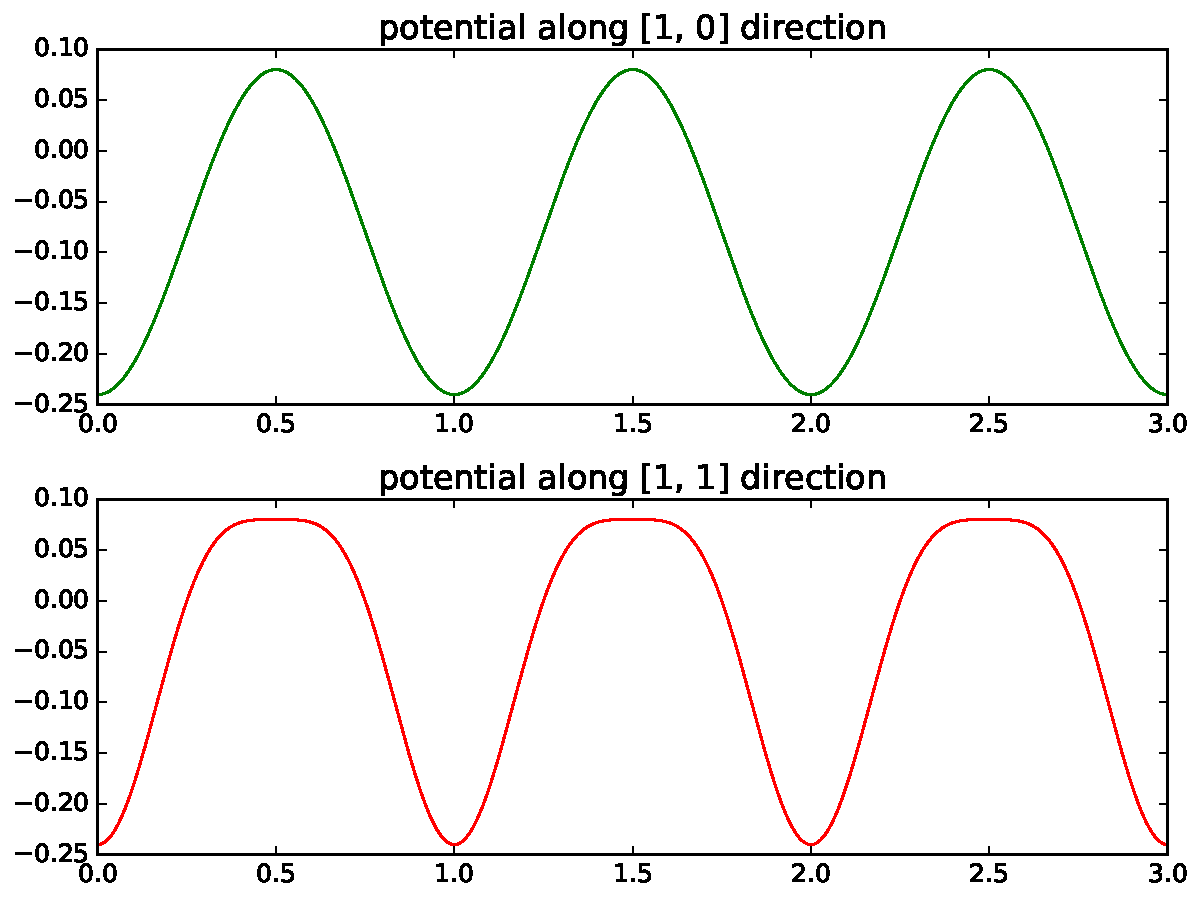
\includegraphics[width=0.7\linewidth]{pro_1.pdf}
	      	\caption{Real space plot of this potential for two separate directions.}
	      	\label{fig:pro1}
	      \end{figure}
	\item We assume $H=H_0 + H_1$, so
	      \begin{equation}
	      	H_0 = \frac{\hbar^2}{2m} (\bm{k} + \bm{G})^2,
	      \end{equation}
	      where $\bm{G} = m_1 \bm{b}_1 + m_2\bm{b}_2$, $m_1$, $m_2 = 0$, $-1$, $1\ldots$, and $\bm{k} = (k_x, k_y)$.
	      To calculate the entry of $H_0$, we already know
	      \begin{equation}
	      	(H_0)_{ij} = \frac{\hbar^2}{2m}(\bm{k} + \bm{G}_j)^2 \delta_{ij},
	      \end{equation}
	      where we suppose
	      \begin{equation}
	      	\begin{aligned}
	      		\bm{G}_1 & = (0,0),    & \bm{G}_2 & = (1,0),   & \bm{G}_3 & = (-1, 0), \\
	      		\bm{G}_4 & = (0,1),    & \bm{G}_5 & = (0, -1), & \bm{G}_6 & = (1,1),   \\
	      		\bm{G}_7 & = (-1, -1), & \bm{G}_8 & = (1,-1),  & \bm{G}_9 & = (-1, 1),
	      	\end{aligned}
	      \end{equation}
	      where $\bm{G} = (m_1, m_2)$ stands for $\bm{G} = m_1 \bm{b}_1 + m_2\bm{b}_2$.
	      Assuming $\bm{k} = (k_x, k_y)$, where $k_x$ and $k_y$ is dimensionless.
	      So we have
	      \begin{equation}
	      	\begin{split}
	      		H_0 & = A
	      		\left(
	      		\begin{smallmatrix}
	      			(\bm{k} + \bm{G}_1)^2 & 0 & 0 & 0 & 0 & 0 & 0 & 0 & 0 \\
	      			0 &  (\bm{k} + \bm{G}_2)^2 & 0 & 0 & 0 & 0 & 0 & 0 & 0 \\
	      			0 & 0 & (\bm{k} + \bm{G}_3)^2 & 0 & 0 & 0 & 0 & 0 & 0 \\
	      			0 & 0 & 0& (\bm{k} + \bm{G}_4)^2 & 0 & 0 & 0 & 0 & 0 \\
	      			0 & 0 & 0 & 0 & (\bm{k} + \bm{G}_5)^2   & 0 & 0 & 0 & 0 \\
	      			0 & 0 & 0 & 0 & 0 & (\bm{k} + \bm{G}_6)^2  & 0 & 0 & 0 \\
	      			0 & 0 & 0 & 0 & 0 & 0 & (\bm{k} + \bm{G}_7)^2  & 0 & 0 \\
	      			0 & 0 & 0 & 0 & 0 & 0 & 0 & (\bm{k} + \bm{G}_8)^2  & 0 \\
	      			0 & 0 & 0 & 0 & 0 & 0 & 0 & 0 &(\bm{k} + \bm{G}_9)^2 \\
	      		\end{smallmatrix}
	      		\right)\\
	      		&=  A
	      		\left(
	      		\begin{smallmatrix}
	      			k_x^2 + k_y^2 & 0 & 0 & 0 & 0 & 0 & 0 & 0 & 0 \\
	      			0 &  (k_x + 1)^2 + k_y^2 & 0 & 0 & 0 & 0 & 0 & 0 & 0 \\
	      			0 & 0 &  (k_x - 1)^2 + k_y^2 & 0 & 0 & 0 & 0 & 0 & 0 \\
	      			0 & 0 & 0& k_x^2 + (k_y + 1)^2 & 0 & 0 & 0 & 0 & 0 \\
	      			0 & 0 & 0 & 0 & k_x^2+(k_y-1)^2   & 0 & 0 & 0 & 0 \\
	      			0 & 0 & 0 & 0 & 0 & (k_x + 1)^2 + (k_y+1)^2  & 0 & 0 & 0 \\
	      			0 & 0 & 0 & 0 & 0 & 0 & (k_x - 1)^2 + (k_y-1)^2  & 0 & 0 \\
	      			0 & 0 & 0 & 0 & 0 & 0 & 0 & (k_x + 1)^2 + (k_y-1)^2  & 0 \\
	      			0 & 0 & 0 & 0 & 0 & 0 & 0 & 0 & (k_x - 1)^2 + (k_y+1)^2 \\
	      		\end{smallmatrix}
	      		\right),
	      	\end{split}
	      \end{equation}
	      where $A=\frac{\hbar^2}{2m} \frac{4\pi^2}{a^2} $.
	      We also know that
	      \begin{equation}
	      	(H_1)_{ij} = V_{\bm{G}_i - \bm{G}_j} = V_{(m_{i1} - m_{j1}, m_{i2} - m_{j2})},
	      \end{equation}
	      So
	      \begin{equation}
	      	\begin{split}
	      		H_1 &=  \frac{\hbar^2}{2m}\frac{4\pi^2}{a^2}
	      		\begin{pmatrix}
	      			V_{(0, 0)}   & V_{(-1, 0)}  & V_{(1, 0)}  & V_{(0, -1)}  & V_{(0, 1)}  & V_{(-1, -1)} & V_{(1, 1)} & V_{(-1, 1)} & V_{(1, -1)} \\
	      			V_{(1, 0)}   & V_{(0, 0)}   & V_{(2, 0)}  & V_{(1, -1)}  & V_{(1, 1)}  & V_{(0, -1)}  & V_{(2, 1)} & V_{(0, 1)}  & V_{(2, -1)} \\
	      			V_{(-1, 0)}  & V_{(-2, 0)}  & V_{(0, 0)}  & V_{(-1, -1)} & V_{(-1, 1)} & V_{(-2, -1)} & V_{(0, 1)} & V_{(-2, 1)} & V_{(0, -1)} \\
	      			V_{(0, 1)}   & V_{(-1, 1)}  & V_{(1, 1)}  & V_{(0, 0)}   & V_{(0, 2)}  & V_{(-1, 0)}  & V_{(1, 2)} & V_{(-1, 2)} & V_{(1, 0)}  \\
	      			V_{(0, -1)}  & V_{(-1, -1)} & V_{(1, -1)} & V_{(0, -2)}  & V_{(0, 0)}  & V_{(-1, -2)} & V_{(1, 0)} & V_{(-1, 0)} & V_{(1, -2)} \\
	      			V_{(1, 1)}   & V_{(0, 1)}   & V_{(2, 1)}  & V_{(1, 0)}   & V_{(1, 2)}  & V_{(0, 0 )}  & V_{(2, 2)} & V_{(0, 2)}  & V_{(2, 0)}  \\
	      			V_{(-1, -1)} & V_{(-2, -1)} & V_{(0, -1)} & V_{(-1, -2)} & V_{(-1, 0)} & V_{(-2, -2)} & V_{(0, 0)} & V_{(-2, 0)} & V_{(0, -2)} \\
	      			V_{(1, -1)}  & V_{(0, -1)}  & V_{(2, -1)} & V_{(1, -2)}  & V_{(1, 0)}  & V_{(0, -2)}  & V_{(2, 0)} & V_{(0, 0)}  & V_{(2, -2)} \\
	      			V_{(-1, 1)}  & V_{(-2, 1)}  & V_{(0, 1)}  & V_{(-1, 0)}  & V_{(-1, 2)} & V_{(-2, 0)}  & V_{(0, 2)} & V_{(-2, 2)} & V_{(0, 0)}
	      		\end{pmatrix}\\
	      		&= \frac{\hbar^2}{2m}\frac{4\pi^2}{a^2}
	      		\begin{pmatrix}
	      			0     & -0.04 & -0.04 & -0.04 & -0.04 & -0.02 & -0.02 & -0.02 & -0.02 \\
	      			-0.04 & 0     & 0     & -0.02 & -0.02 & -0.04 & 0     & -0.04 & 0     \\
	      			-0.04 & 0     & 0     & -0.02 & -0.02 & 0.    & -0.04 & 0     & -0.04 \\
	      			-0.04 & -0.02 & -0.02 & 0     & 0     & -0.04 & 0     & 0     & -0.04 \\
	      			-0.04 & -0.02 & -0.02 & 0     & 0     & 0     & -0.04 & -0.04 & 0     \\
	      			-0.02 & -0.04 & 0     & -0.04 & 0     & 0     & 0     & 0     & 0     \\
	      			-0.02 & 0     & -0.04 & 0     & -0.04 & 0     & 0     & 0     & 0     \\
	      			-0.02 & -0.04 & 0     & 0     & -0.04 & 0     & 0     & 0     & 0     \\
	      			-0.02 & 0     & -0.04 & -0.04 & 0     & 0     & 0     & 0     & 0     \\
	      		\end{pmatrix}.
	      	\end{split}
	      \end{equation}
	      Here $H_0$ is the kinetic energy, $H_1$ is the potential. Because we only truncate $9$ $\bm{G}$s,
	      so we assume $V_{(2, *)} = V_{(-2, *)} = V_{(*,-2)} = V_{(*, 2)} = 0$.
	\item Fig.\ \ref{fig:pro31} is eigenvalues with perturbation, Fig.\ \ref{fig:pro32} is free electrons case.
	      \begin{figure}[h]
	      	\centering
	      	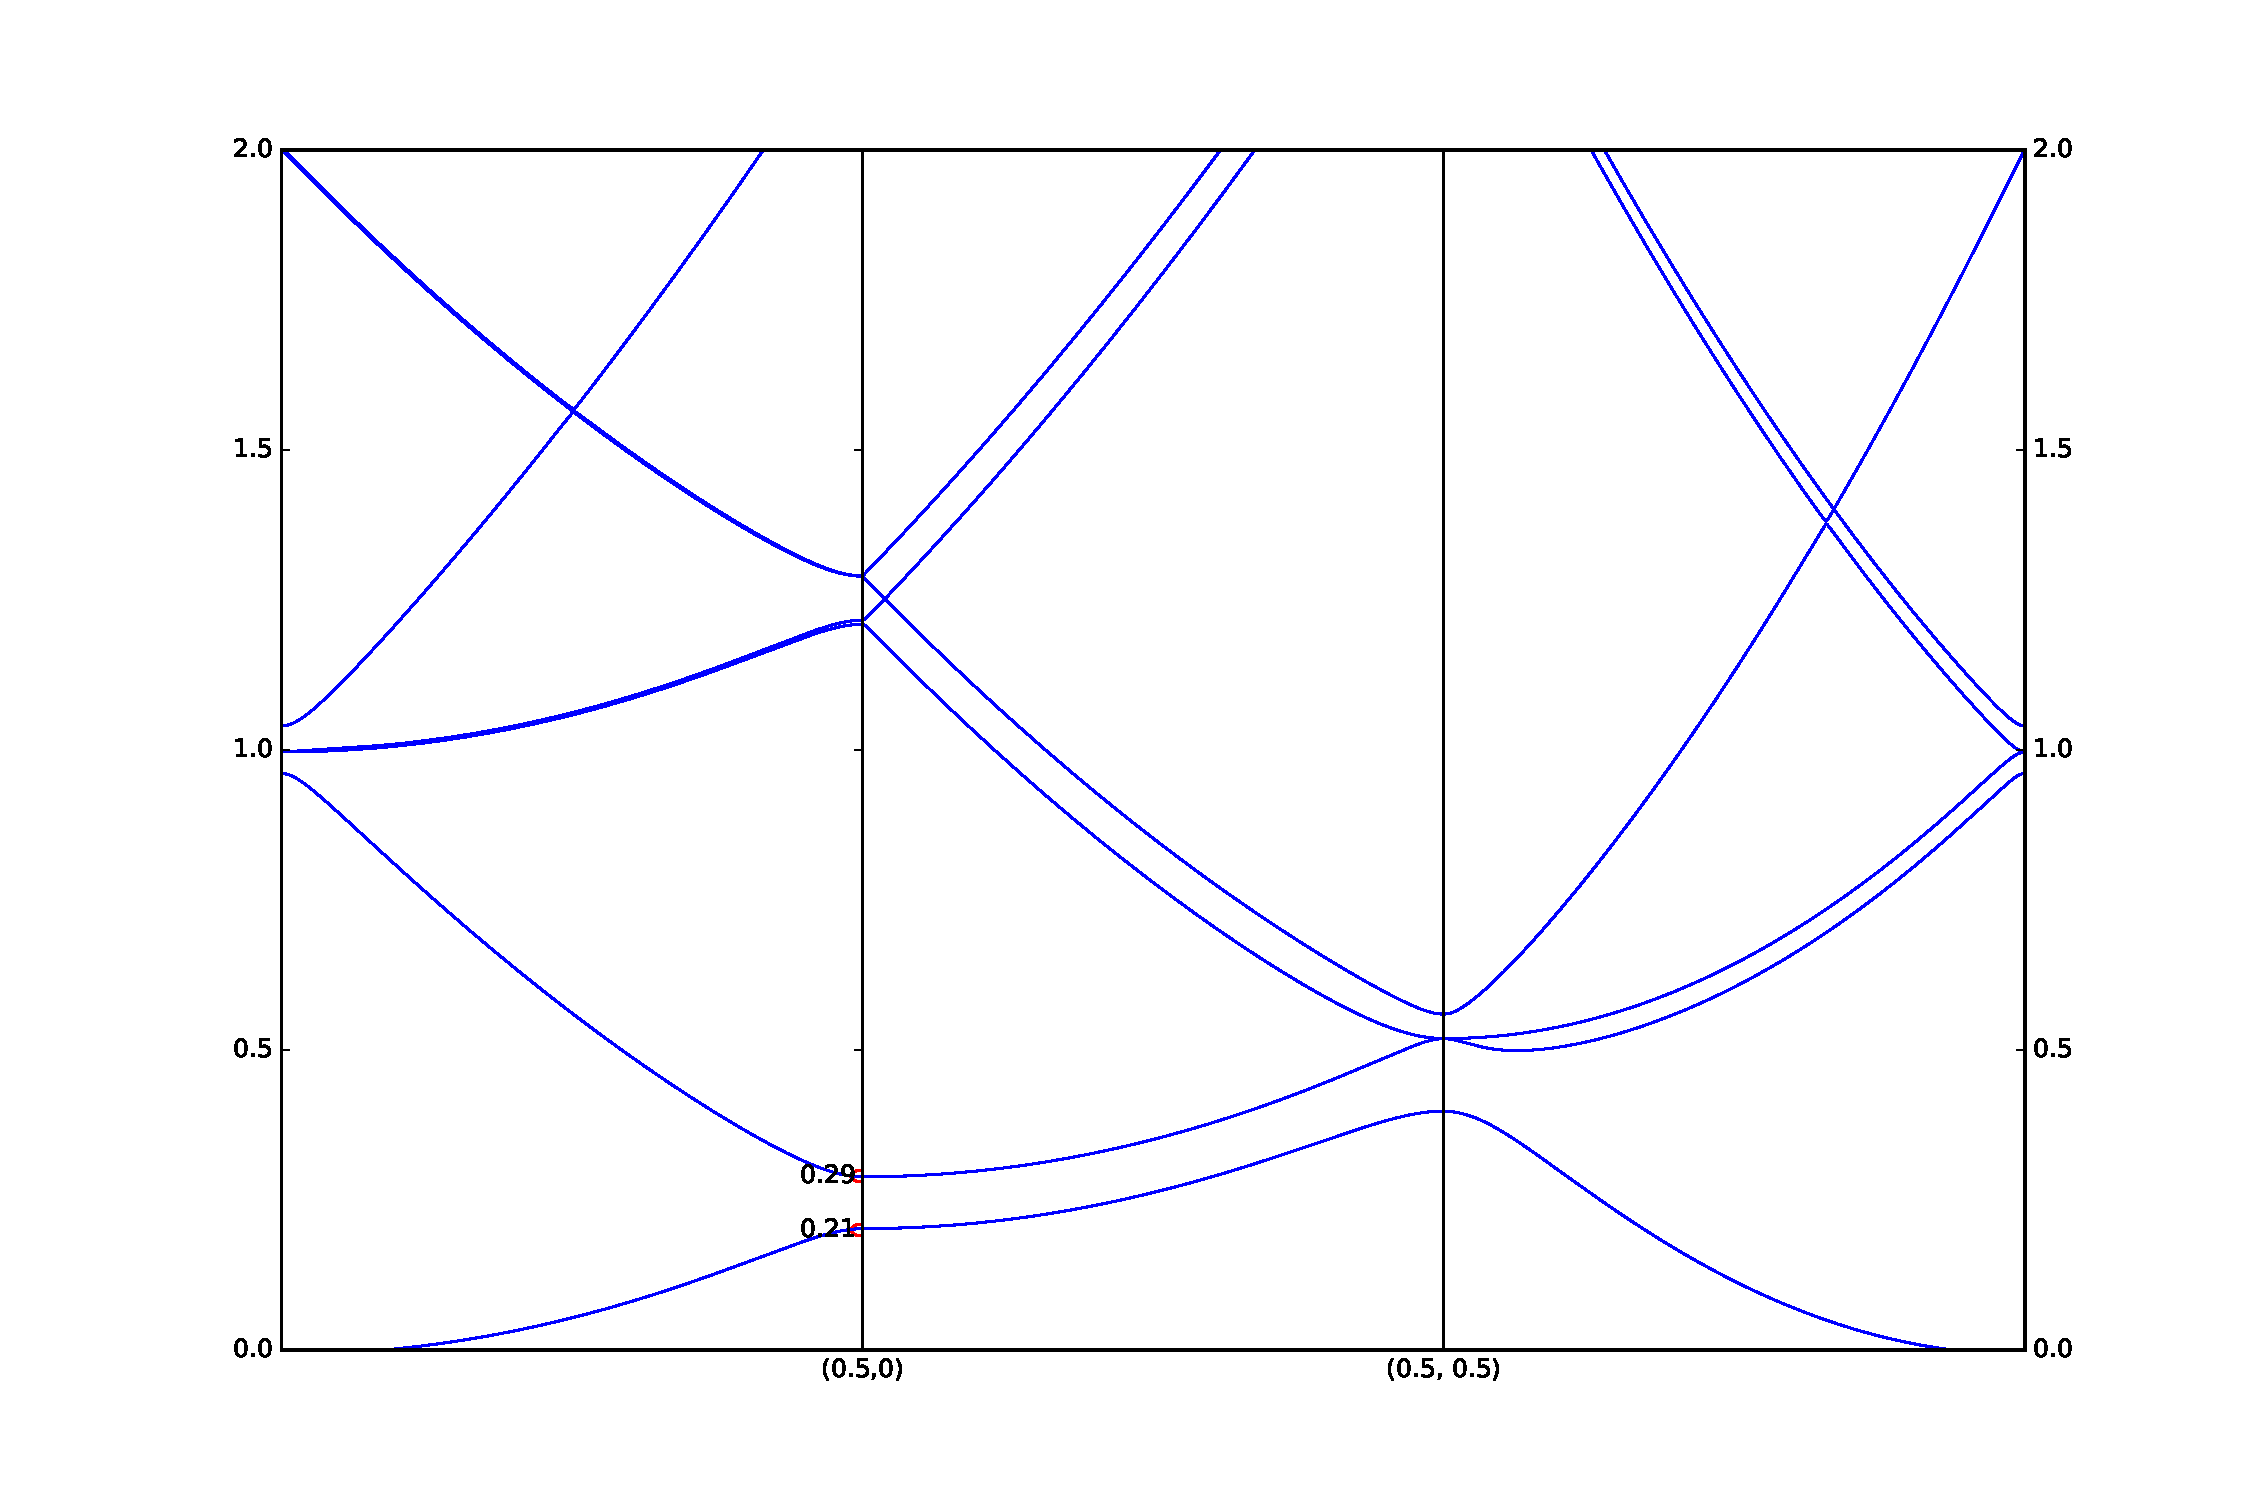
\includegraphics[width=0.8\linewidth]{pro_3_1.pdf}
	      	\caption{Eigenvalues along the path with perturbation.}
	      	\label{fig:pro31}
	      \end{figure}
	      \begin{figure}[h]
	      	\centering
	      	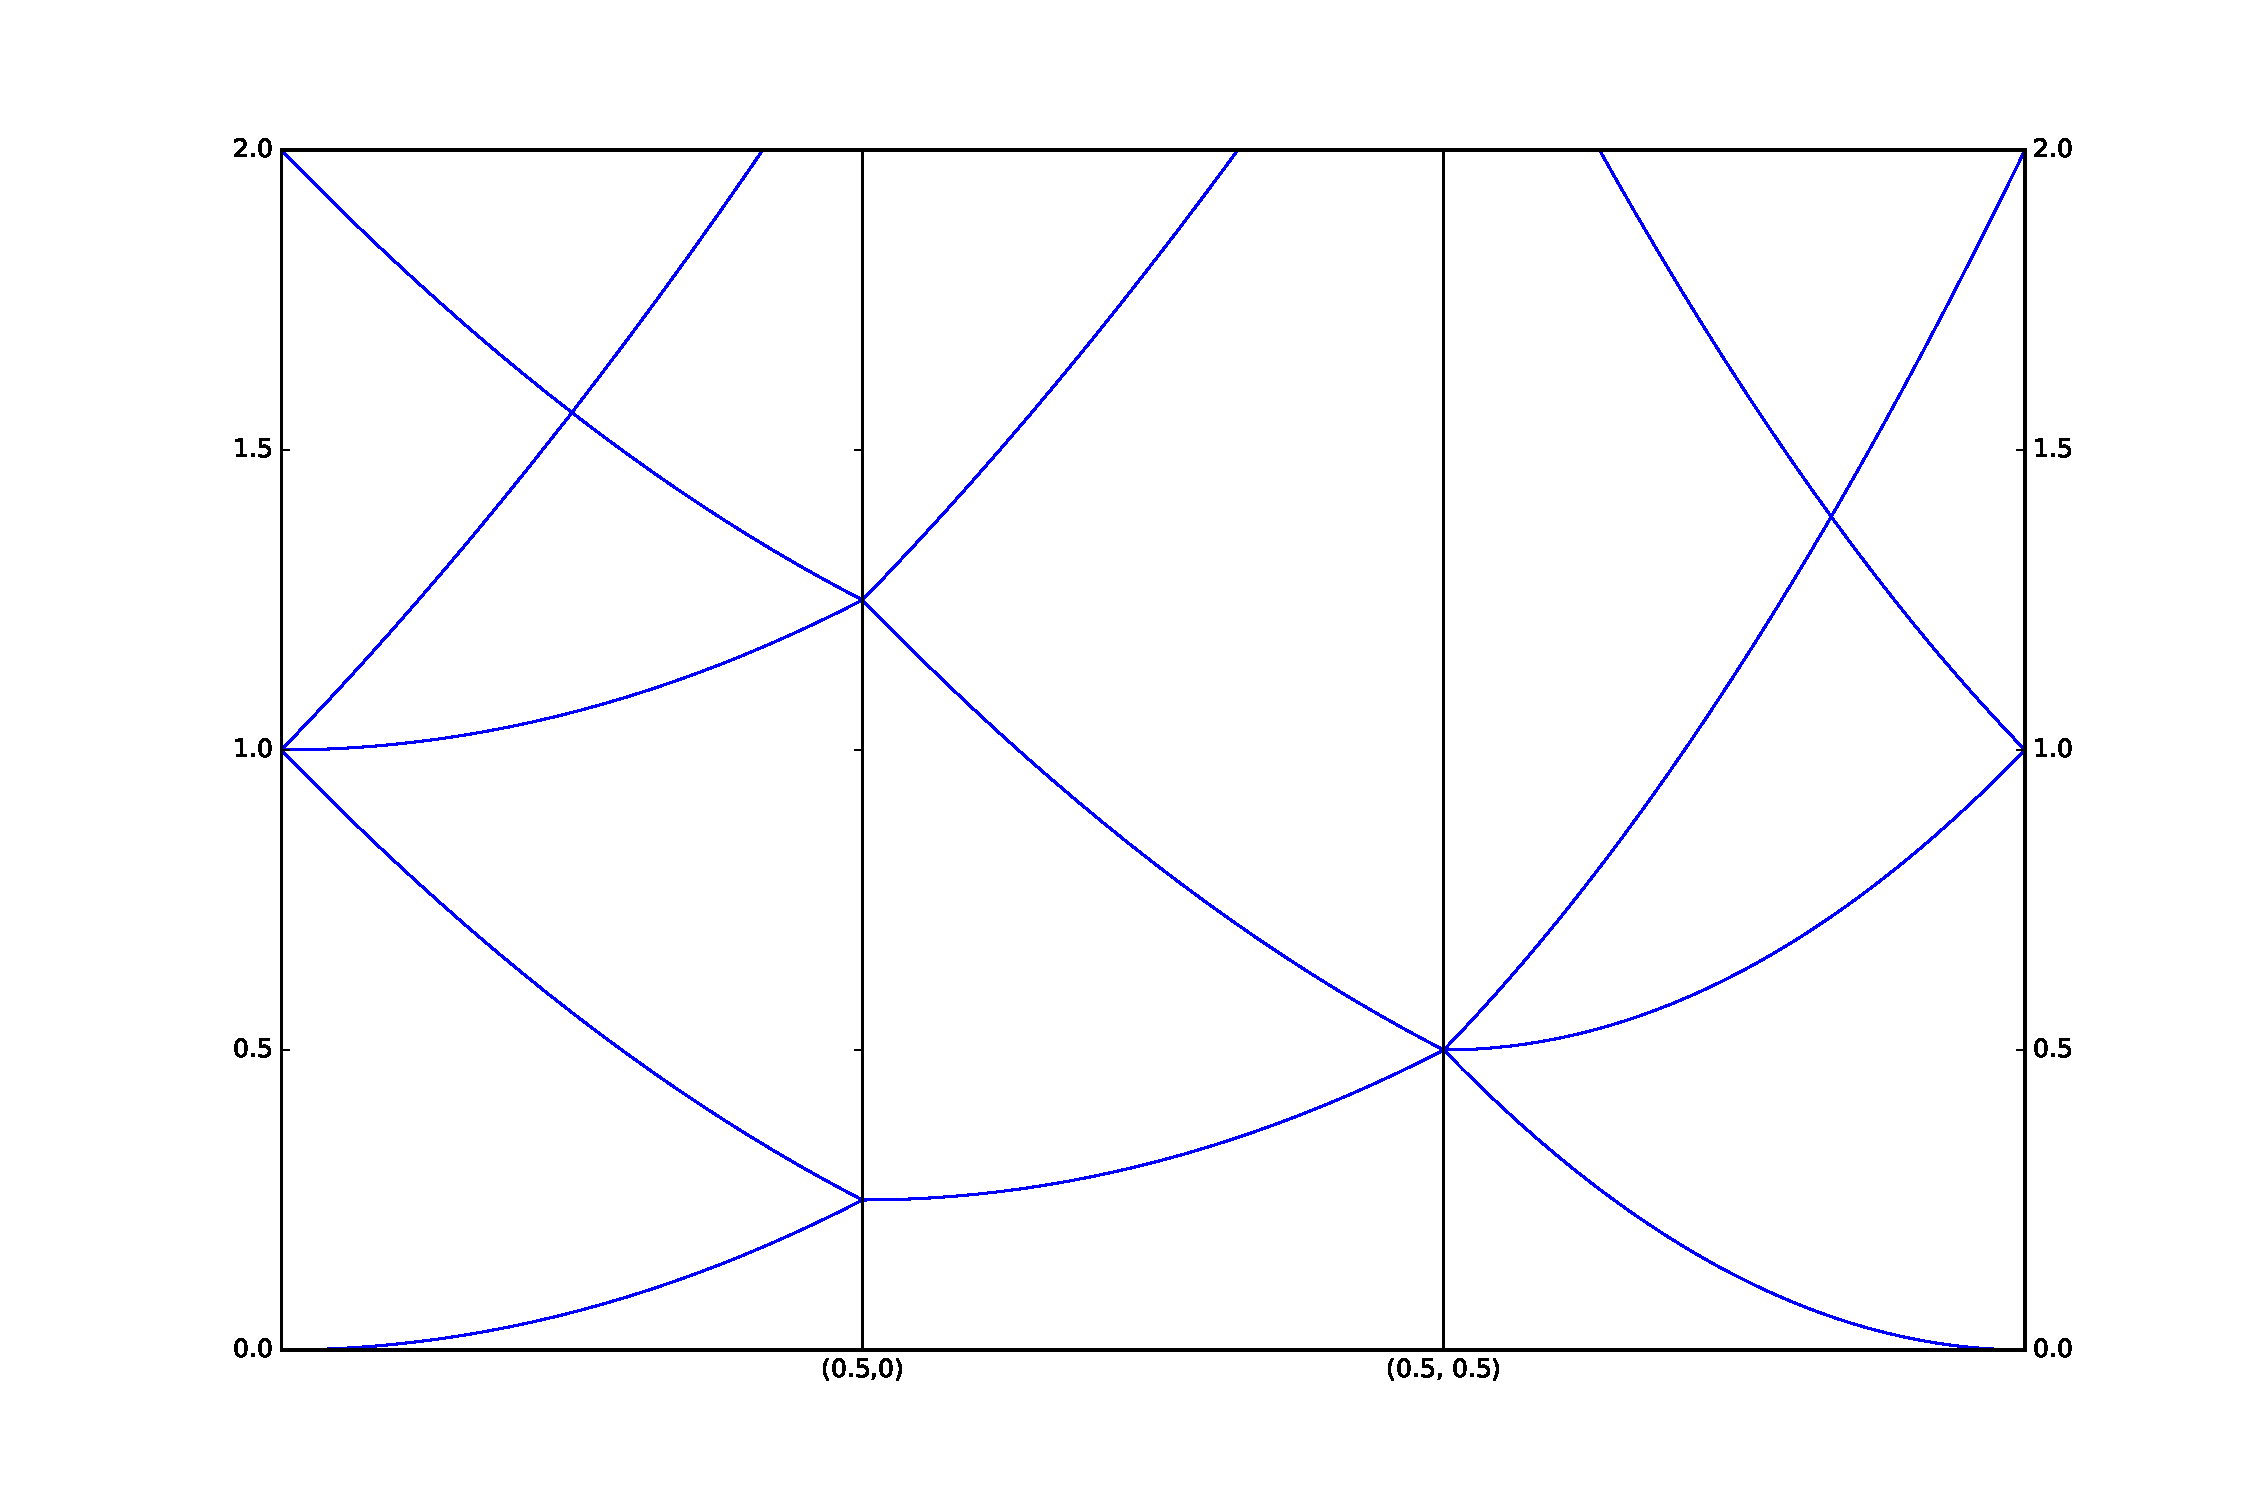
\includegraphics[width=0.8\linewidth]{pro_3_2.pdf}
	      	\caption{Free electrons case.}
	      	\label{fig:pro32}
	      \end{figure}
	\item To truncate only $2$ states, from last homework, we know that $\bm{G}_1 = (0, 0)$ and
	      $\bm{G}_3 = (-1, 0)$ that form the lowest $2$ eigenvalues. So we chose them.

	      \begin{equation}
	      	H_0 = \frac{\hbar^2}{2m}\frac{4\pi^2}{a^2}
	      	\begin{pmatrix}
	      		k_x^2 + k_y^2 & 0                   \\
	      		0             & (k_x - 1)^2 + k_y^2
	      	\end{pmatrix}.
	      \end{equation}
	      And
	      \begin{equation}
	      	H_1 = \frac{\hbar^2}{2m}\frac{4\pi^2}{a^2}
	      	\begin{pmatrix}
	      		0     & -0.04 \\
	      		-0.04 & 0
	      	\end{pmatrix}.
	      \end{equation}
	      Thus
	      \begin{equation}
	      	H =H_0 +H_1 = \frac{\hbar^2}{2m}\frac{4\pi^2}{a^2}
	      	\begin{pmatrix}
	      		k_x^2 + k_y^2 & -0.04               \\
	      		-0.04         & (k_x - 1)^2 + k_y^2
	      	\end{pmatrix}.
	      \end{equation}
	      To have non-trivial solutions, we need $\det (H) = 0$.
	      That is to say,
	      \begin{equation}
	      	\begin{vmatrix}
	      		k_x^2 + k_y^2 -\varepsilon & -0.04                            \\
	      		-0.04                      & (k_x - 1)^2 + k_y^2 -\varepsilon
	      	\end{vmatrix} = 0.
	      \end{equation}
	      With $k_x = 0.5$, $k_y = 0$,
	      then we derive $\varepsilon_1 = 0.21\times \frac{\hbar^2}{2m}\frac{4\pi^2}{a^2}$ or $\varepsilon_2 = 0.29\times \frac{\hbar^2}{2m}\frac{4\pi^2}{a^2}$, which can be seen from Fig.\ \ref{fig:pro31}.
	\item There is one degeneracy remaining, at position $(0.5, 0.5)$, whose eigenvalue is approximate to $0.5189\times \frac{\hbar^2}{2m}\frac{4\pi^2}{a^2}$. The size is $2$-fold.
\end{enumerate}

\end{document}
